\begin{figure}[t]
\newcommand{\figwidth}{1.7in}
\begin{center}
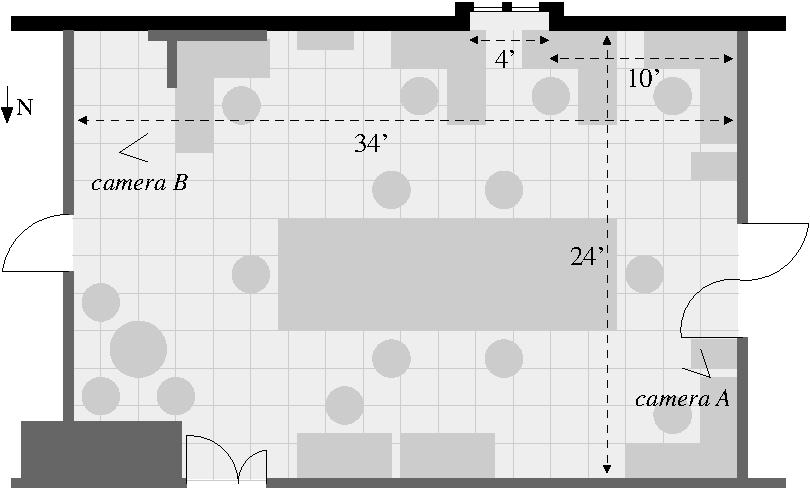
\includegraphics[width=2.5in]{lab.pdf} \vspace{0.1in}
\\
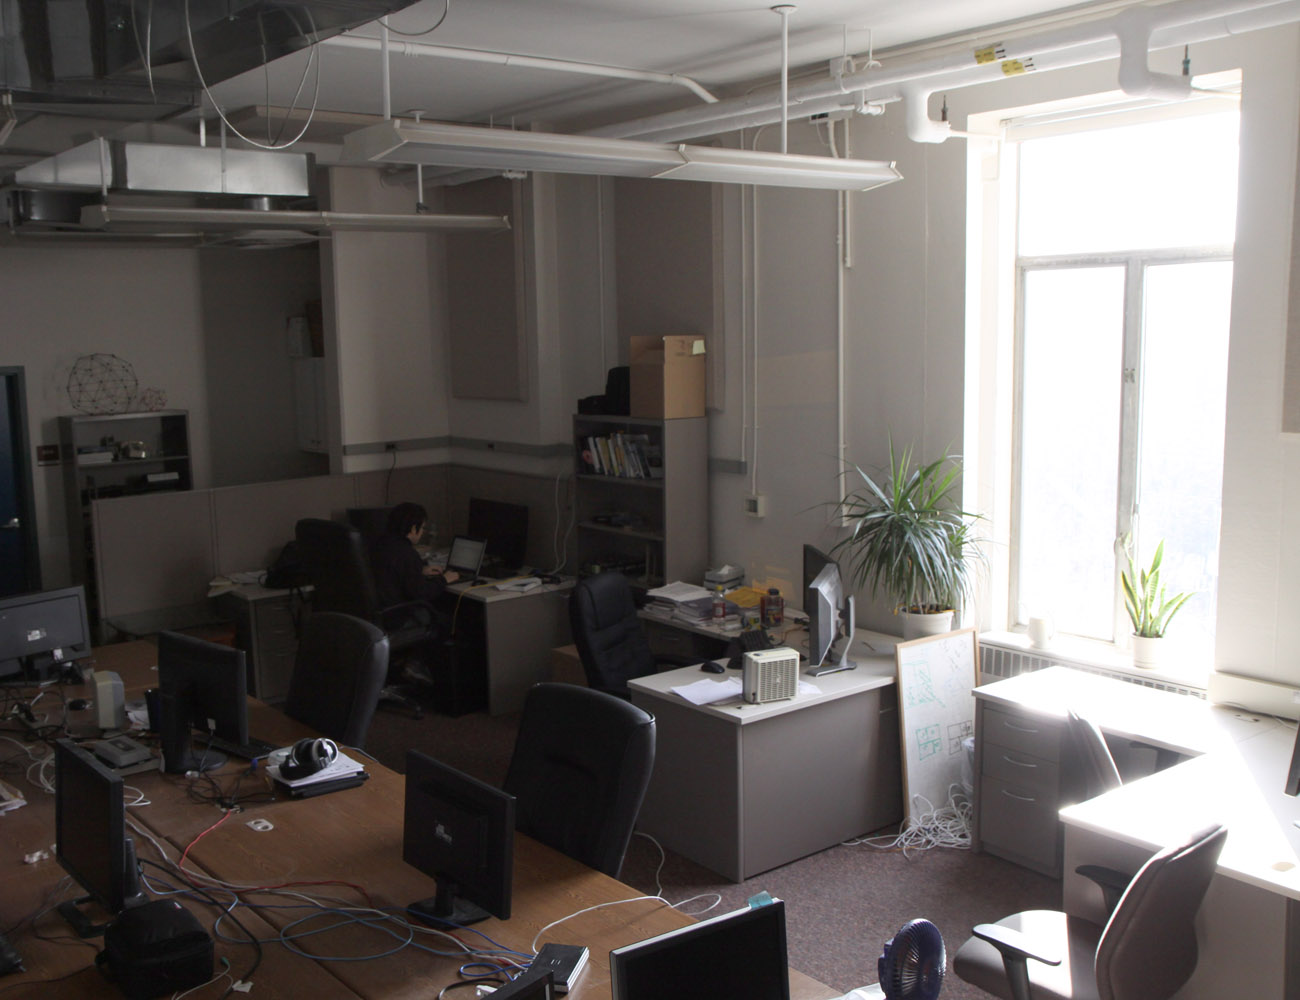
\includegraphics[width=\figwidth]{camera_angle_2_lights_off}
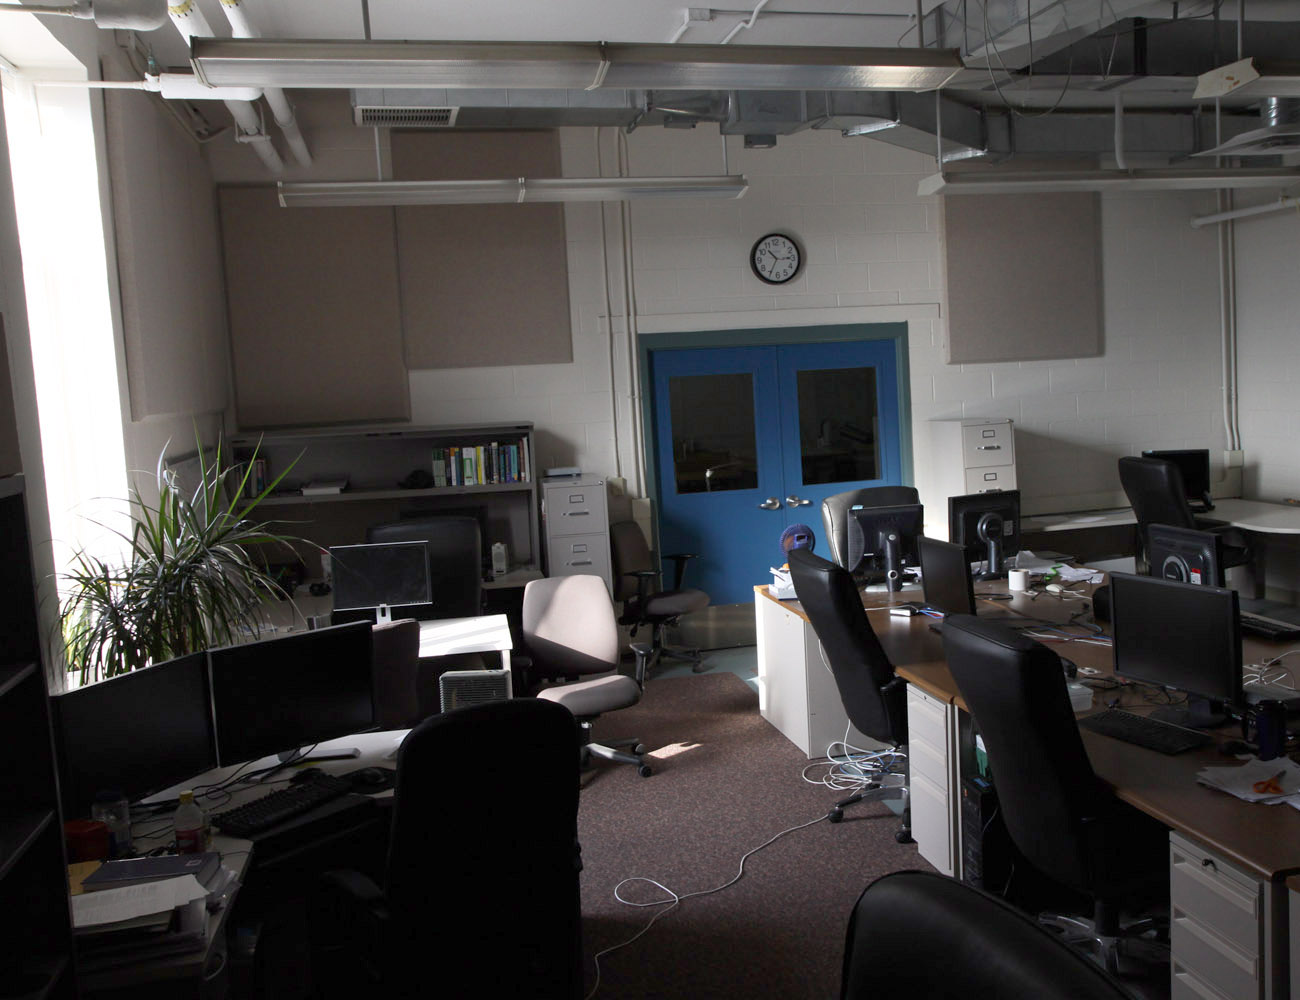
\includegraphics[width=\figwidth]{camera_angle_3_lights_off}\vspace{-0.21in}\\
\begin{minipage}{\figwidth}~{\color{white}{\em camera A}}\end{minipage}
\begin{minipage}{\figwidth}~{\color{white}{\em camera B}}\end{minipage}\vspace{-0.05in}\\
%\begin{minipage}{\figwidth}~{\color{white}{\em camera B, lights on}}\end{minipage}%\vspace{0.00in}\\
\caption{User study participants visited this simple open office
  environment as a case study for daylighting analysis.  The room
  contains a single, tall and narrow, south-facing window that
  provides direct overly-intense illumination to portions of the room
  while leaving other areas relatively dark.  Thus, occupants of the
  space typically turn on the overhead lights, and on sunny afternoons
  a diffusing shade is needed to prevent glare.
% even on sunny
%  afternoons.
\label{figure:example_room}
}
\end{center}
\end{figure}
